\section{Preliminaries}
\label{sec:pre}
Let $\{\cdot\}$ denote sets and $\{\!\!\{\cdot\}\!\!\}$  multisets. 
We consider undirected simple graphs $G = (V, E)$ where $V$ is the vertex set and $E$ is the edge set. 
We use $\lvert\cdot\rvert$ to denote the cardinality of a set/multiset/sequence, $e_{vu} = \{v,u\}$ an undirected edge connecting vertices $v$ and $u$, and $\vec{e}_{vu} = (v,u)$ a directed edge that starts from vertex $v$ and ends at vertex $u$. Thus, $e_{vu} = e_{uv}$ and $\vec{e}_{vu} \neq \vec{e}_{uv}$. We use $d(v,u)$ to denote the shortest-path distance between vertices $v$ and $u$.
A \emph{$\delta$-neighborhood} of a vertex $v$ is a set of vertices within the distance $\delta$ from $v$, i.e. $N_{\delta}(v)=\{u\in V:1\leq d(v,u)\leq \delta\}$.
A path $\mathcal{P}_{w_0w_k}$ of length $k$ in $G$, called \emph{k-path}, is a sequence $(w_0, w_1, ..., w_k)$ of distinct vertices such that $(w_{i-1}, w_{i}) \in E$ for $i=1,2,...,k$. 
% An empty path $()$ is allowed. A path $\mathcal{P}'$ is a \emph{subpath} of $\mathcal{P}$, denoted $\mathcal{P}' \vartriangleleft \mathcal{P}$, if $\mathcal{P}'=(w'_0, w'_1, ..., w'_{k'})$ is a contiguous subsequence of $(w_0, w_1, ..., w_k)$. That is, for $0\leq i\leq i+k'\leq k$ we have $w'_0=w_i,w'_1=w_{i+1},...,w'_{k'}=w_{i+k'}$. Respectively, we call $\mathcal{P}$ a \emph{superpath} of $\mathcal{P}'$, denoted $\mathcal{P} \triangleright \mathcal{P}'$. %A path of length $k$ is called a k-path.
% A path $\mathcal{P}$ can also be expressed as a sequence of consecutive directed edges $\mathcal{P} = (\vec{e}_{w_0w_1}, \vec{e}_{w_1w_2},..., \vec{e}_{w_{k-1}w_{k}})$.
% If $w_1$ precedes $w_2$ on $\mathcal{P}$, we denote it as $(w_1\prec w_2)_\mathcal{P}$.

\paragraph{Graph searching.} 
Graph traversal, or \emph{graph searching}, visits each vertex in a graph. \emph{Breadth-First Search} (BFS) and \emph{Depth-First Search} (DFS) are the two most widely used graph search algorithms, which differ in the order of visiting vertices. Both methods start at a vertex $v$. BFS first visits the direct neighbours in $N_1(v)$ of $v$ and then the neighbours in $N_2(v)$ that have not been visited, etc. The idea is to process all vertices in $N_i$ of distance (or level) $i$ from $v$ before processing vertices at level $i+1$ or greater. The process is repeated until all vertices reachable from $v$ have been visited. In DFS we instead go as ``deep" as possible from vertex $v$ until no new vertices can be visited. Then we backtrack and try other neighbours that were missed from the farthest in the search paths until all vertices are visited. The visited vertices and the edges along the search paths form a BFS/DFS search tree. For example, the solid lines in \cref{subfig:edge_type_b,subfig:edge_type_c} represent two different search trees for the graph in \cref{subfig:edge_type_a}. Given a graph, generally, there are many ways to construct different search trees by selecting different starting points and different edges to visit vertices.

\paragraph{Visiting order subscripting.} Vertices being visited in a graph search form a linear order. We use subscripts to label this order based on their discovery/first-visited time~\citep{Cormen_algointro}. Given a search tree, we say $v_i$ \emph{precedes} $v_j$, denoted as $v_i\prec v_j$, if $v_i$ is discovered before $v_j$. $i$ and $j$ are subscripts that indicate the relation: for all $i$ and $j$, $v_i\prec v_j$ if and only if $i< j$. Each vertex is discovered once, so a subscript ranges from 0 to $N-1$ in a graph $G$. $v_0$ is called the root. \cref{fig:edge_type} shows how the subscripting is used to indicate vertex visiting orders. 

% \q{(it sounds the subscripts for vertices are defined w.r.t. a BFS/DFS search on the whole graph $G$ but you intend to apply BFS/DFS on subgraphs. a vertex may appear in multiple subgraphs, so using subscripts could be confusing.)}

\paragraph{Tree and back edges.} For an undirected simple graph $G=(V,E)$, BFS/DFS categorise the edges in $E$ into \emph{tree edges} and \emph{back edges}. 

Tree edges and back edges are both directed, i.e., $(v,u)\neq (u,v)$. Let $T_v$ denote a search tree rooted at vertex $v$. A tree edge is an edge in the search tree $T_v$, starting from an early-visited vertex to a later-visited vertex. A back edge starts from a later-visited vertex to an early-visited vertex.
A directed edge $(v_i, v_j)$ is either a tree edge (if $i<j$), or a back edge (if $i>j$).
For example, dashed lines in \cref{subfig:edge_type_b,subfig:edge_type_c} represent back edges in BFS and DFS search trees, respectively. 
In BFS, a back edge $(v_i, v_j)$ connects vertices at the same or adjacent level, i.e. $d(v_0,v_i) =d(v_0,v_j)$ or $|d(v_0,v_i) - d(v_0,v_j)| = 1$~\citep{Cormen_algointro}. For this reason back edges in BFS are sometimes referred to as \emph{cross edges}.
In DFS, a back edge $(v_i,v_j)$ connects a vertex $v_i$ and its non-parent ancestor $v_j$; therefore we always have $v_j\prec v_i$ (or $i>j$). 

We use $E_{\text{tree}}^{T_v}$ and $E_{\text{back}}^{T_v}$ to denote the tree edge set and the back edge set with respect to a search tree $T_v$ rooted at $v$. 

% Sean Revised here

% We denote $E_{\text{tree}} = \{\vec{e} : \forall i,j, i< j, \vec{e}=(v_i,v_j), \{v_i,v_j\}\in E\}$ as the tree edge set in $G$, and $E_{\text{back}} = \{\vec{e} : \forall i,j, i> j, \vec{e}=(v_i,v_j), \{v_i,v_j\}\in E\}$ as the back edge set in $G$.

% For a given root vertex $v$, there is a path from the root vertex $v$ formed by tree edges to every other vertex in a search tree. These paths form a path set $\mathbb{P}_v = \{\mathcal{P}_{vw_1}, \mathcal{P}_{vw_2}, ..., \mathcal{P}_{vw_n}\}$ where $w_i\in V\backslash\{v\}$ is the ending vertex of the path $\mathcal{P}_{vw_i}$. When the search range is limited to $N_{\delta}(v)$, the corresponding path set is denoted as $\mathbb{P}_{v,\delta}$.



% \paragraph{Problem setting.} This paper focuses on the following three problems. Firstly, we study an alternative vertex colouring architecture guided by graph searching, which is strictly more expressive than 1-WL test and more efficient than higher-order WL tests. Secondly, we study the graph and subgraph properties that different graph-searching strategies can capture in the proposed vertex colouring, and how these properties can improve expressivity. Lastly, we study how search radius influences model expressivity.


\begin{figure}[t]
\centering
\begin{subfigure}{.3\columnwidth}
\captionsetup{width=.3\columnwidth}
        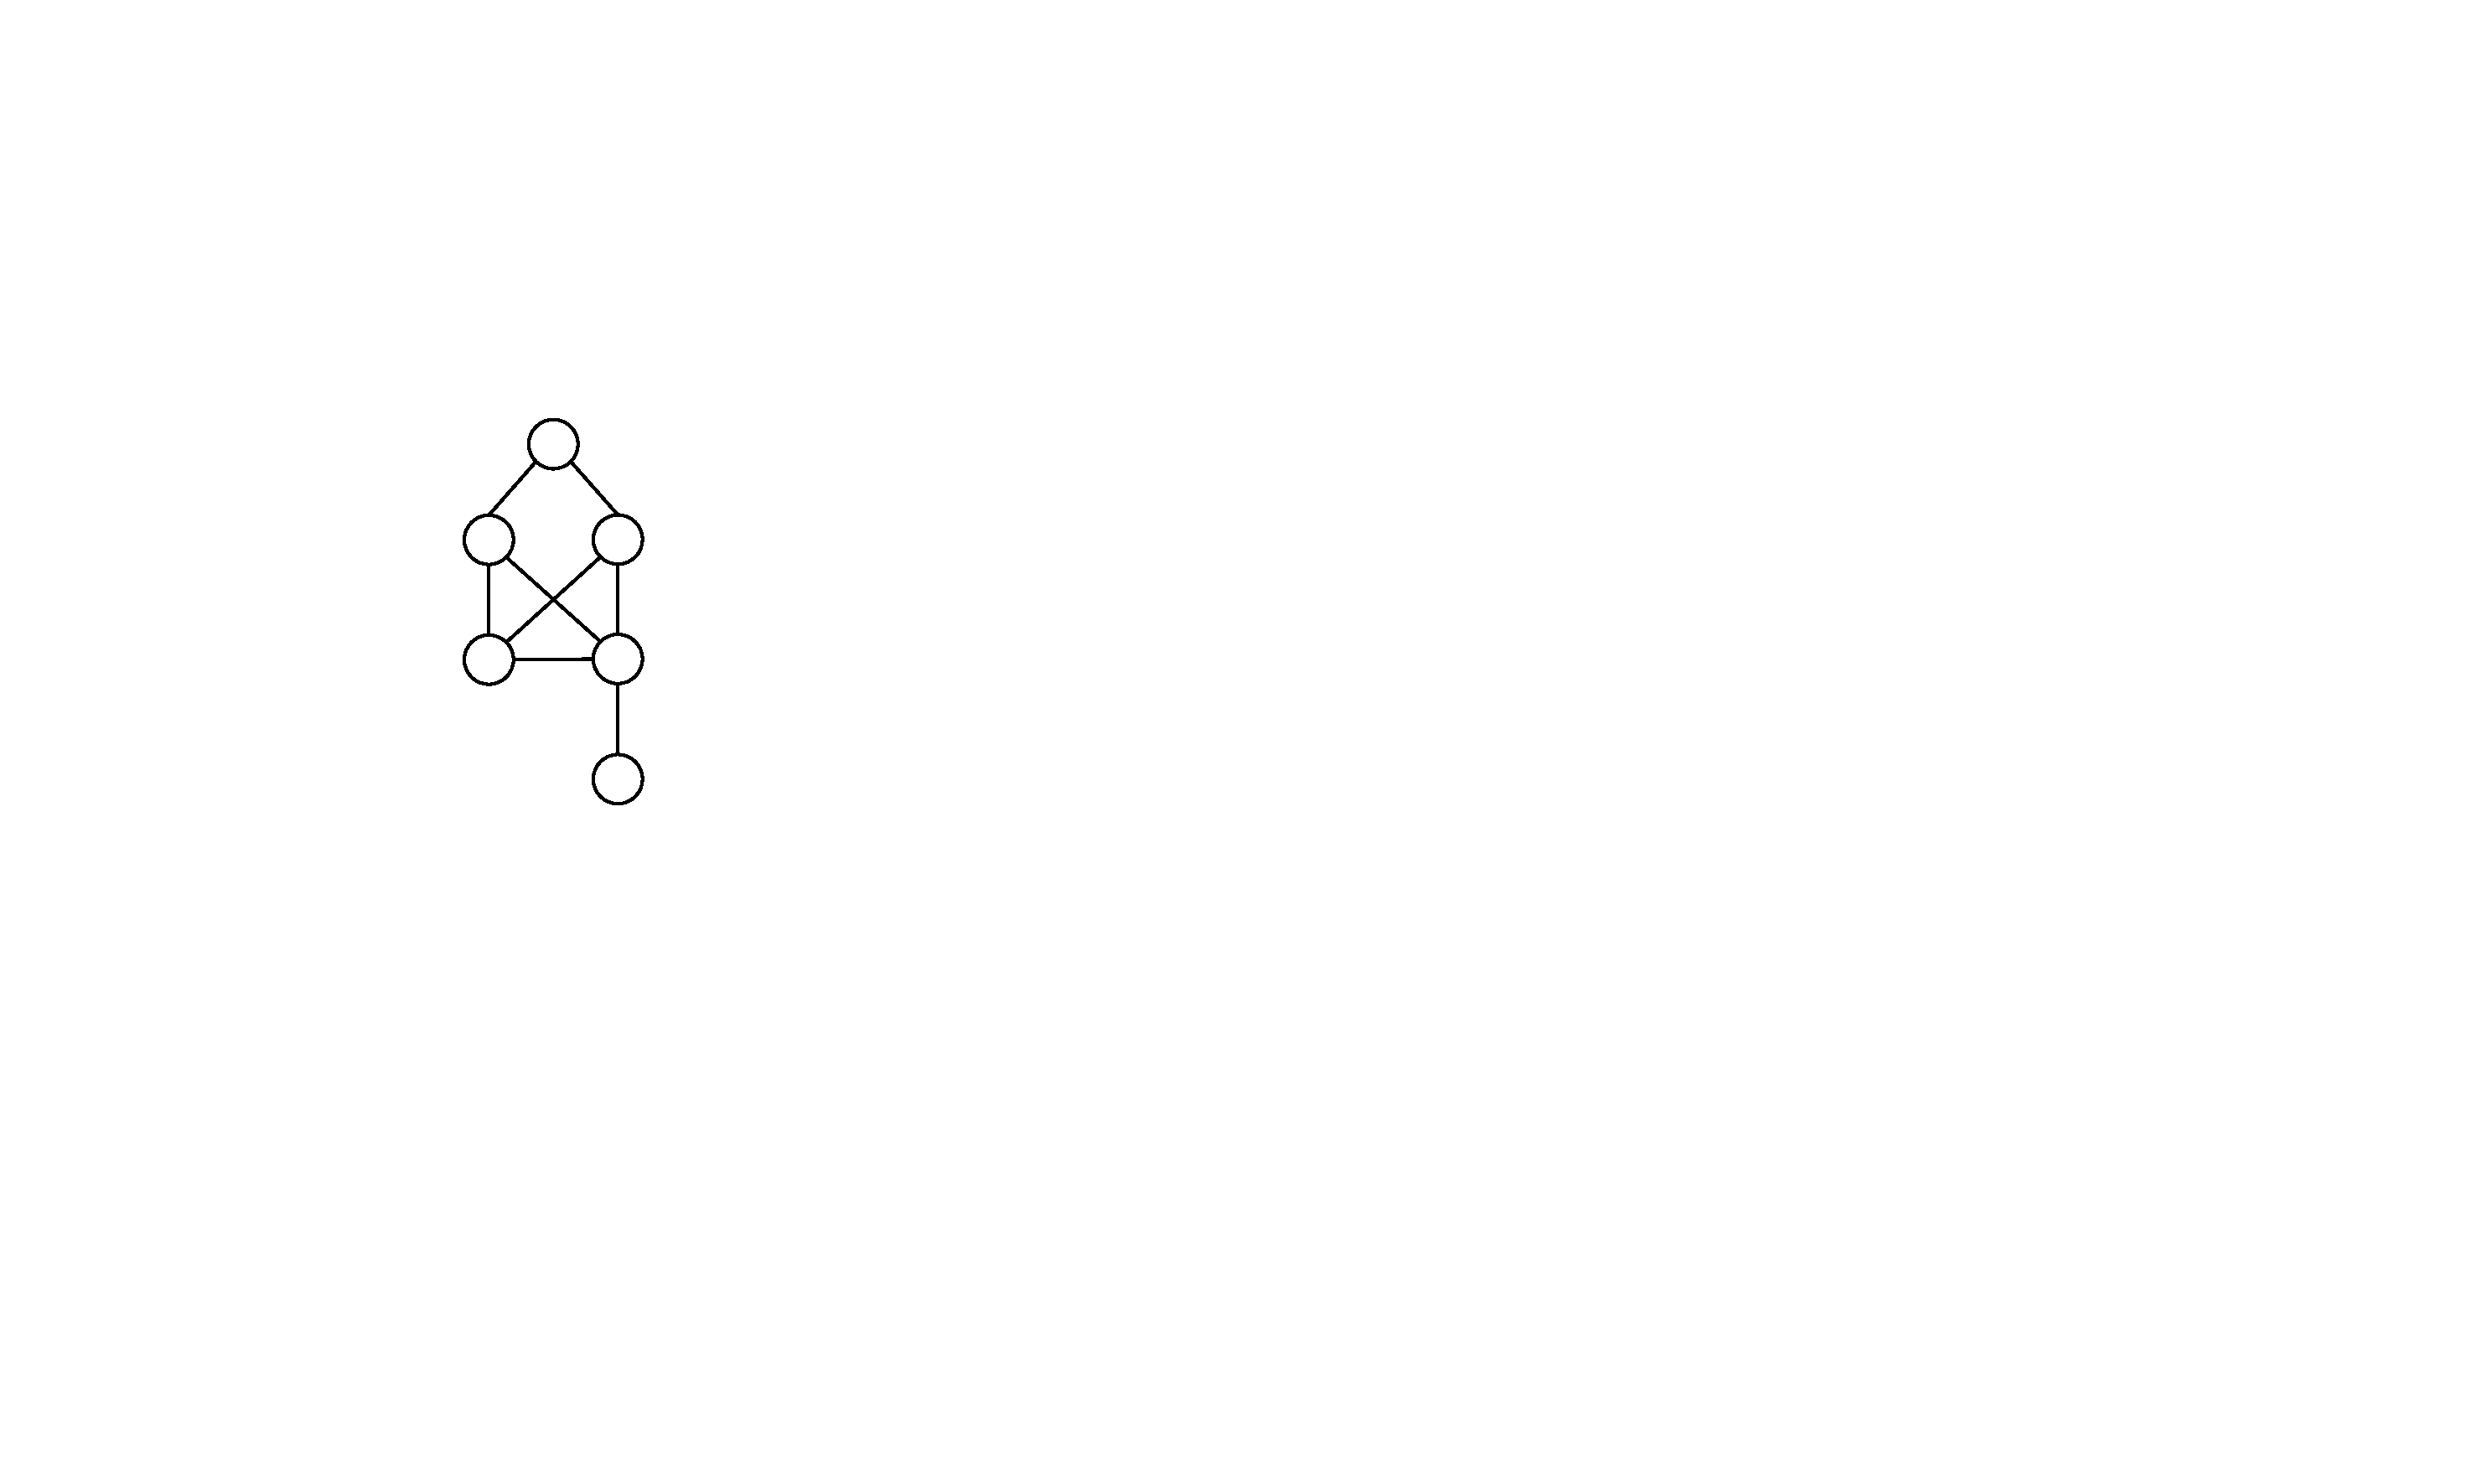
\includegraphics[clip,width=\textwidth]{figures/edge_type_a_new.pdf}
\subcaption{}
\label{subfig:edge_type_a}
\end{subfigure}%
\hfill
\begin{subfigure}{.3\columnwidth}
\captionsetup{width=.9\linewidth}
        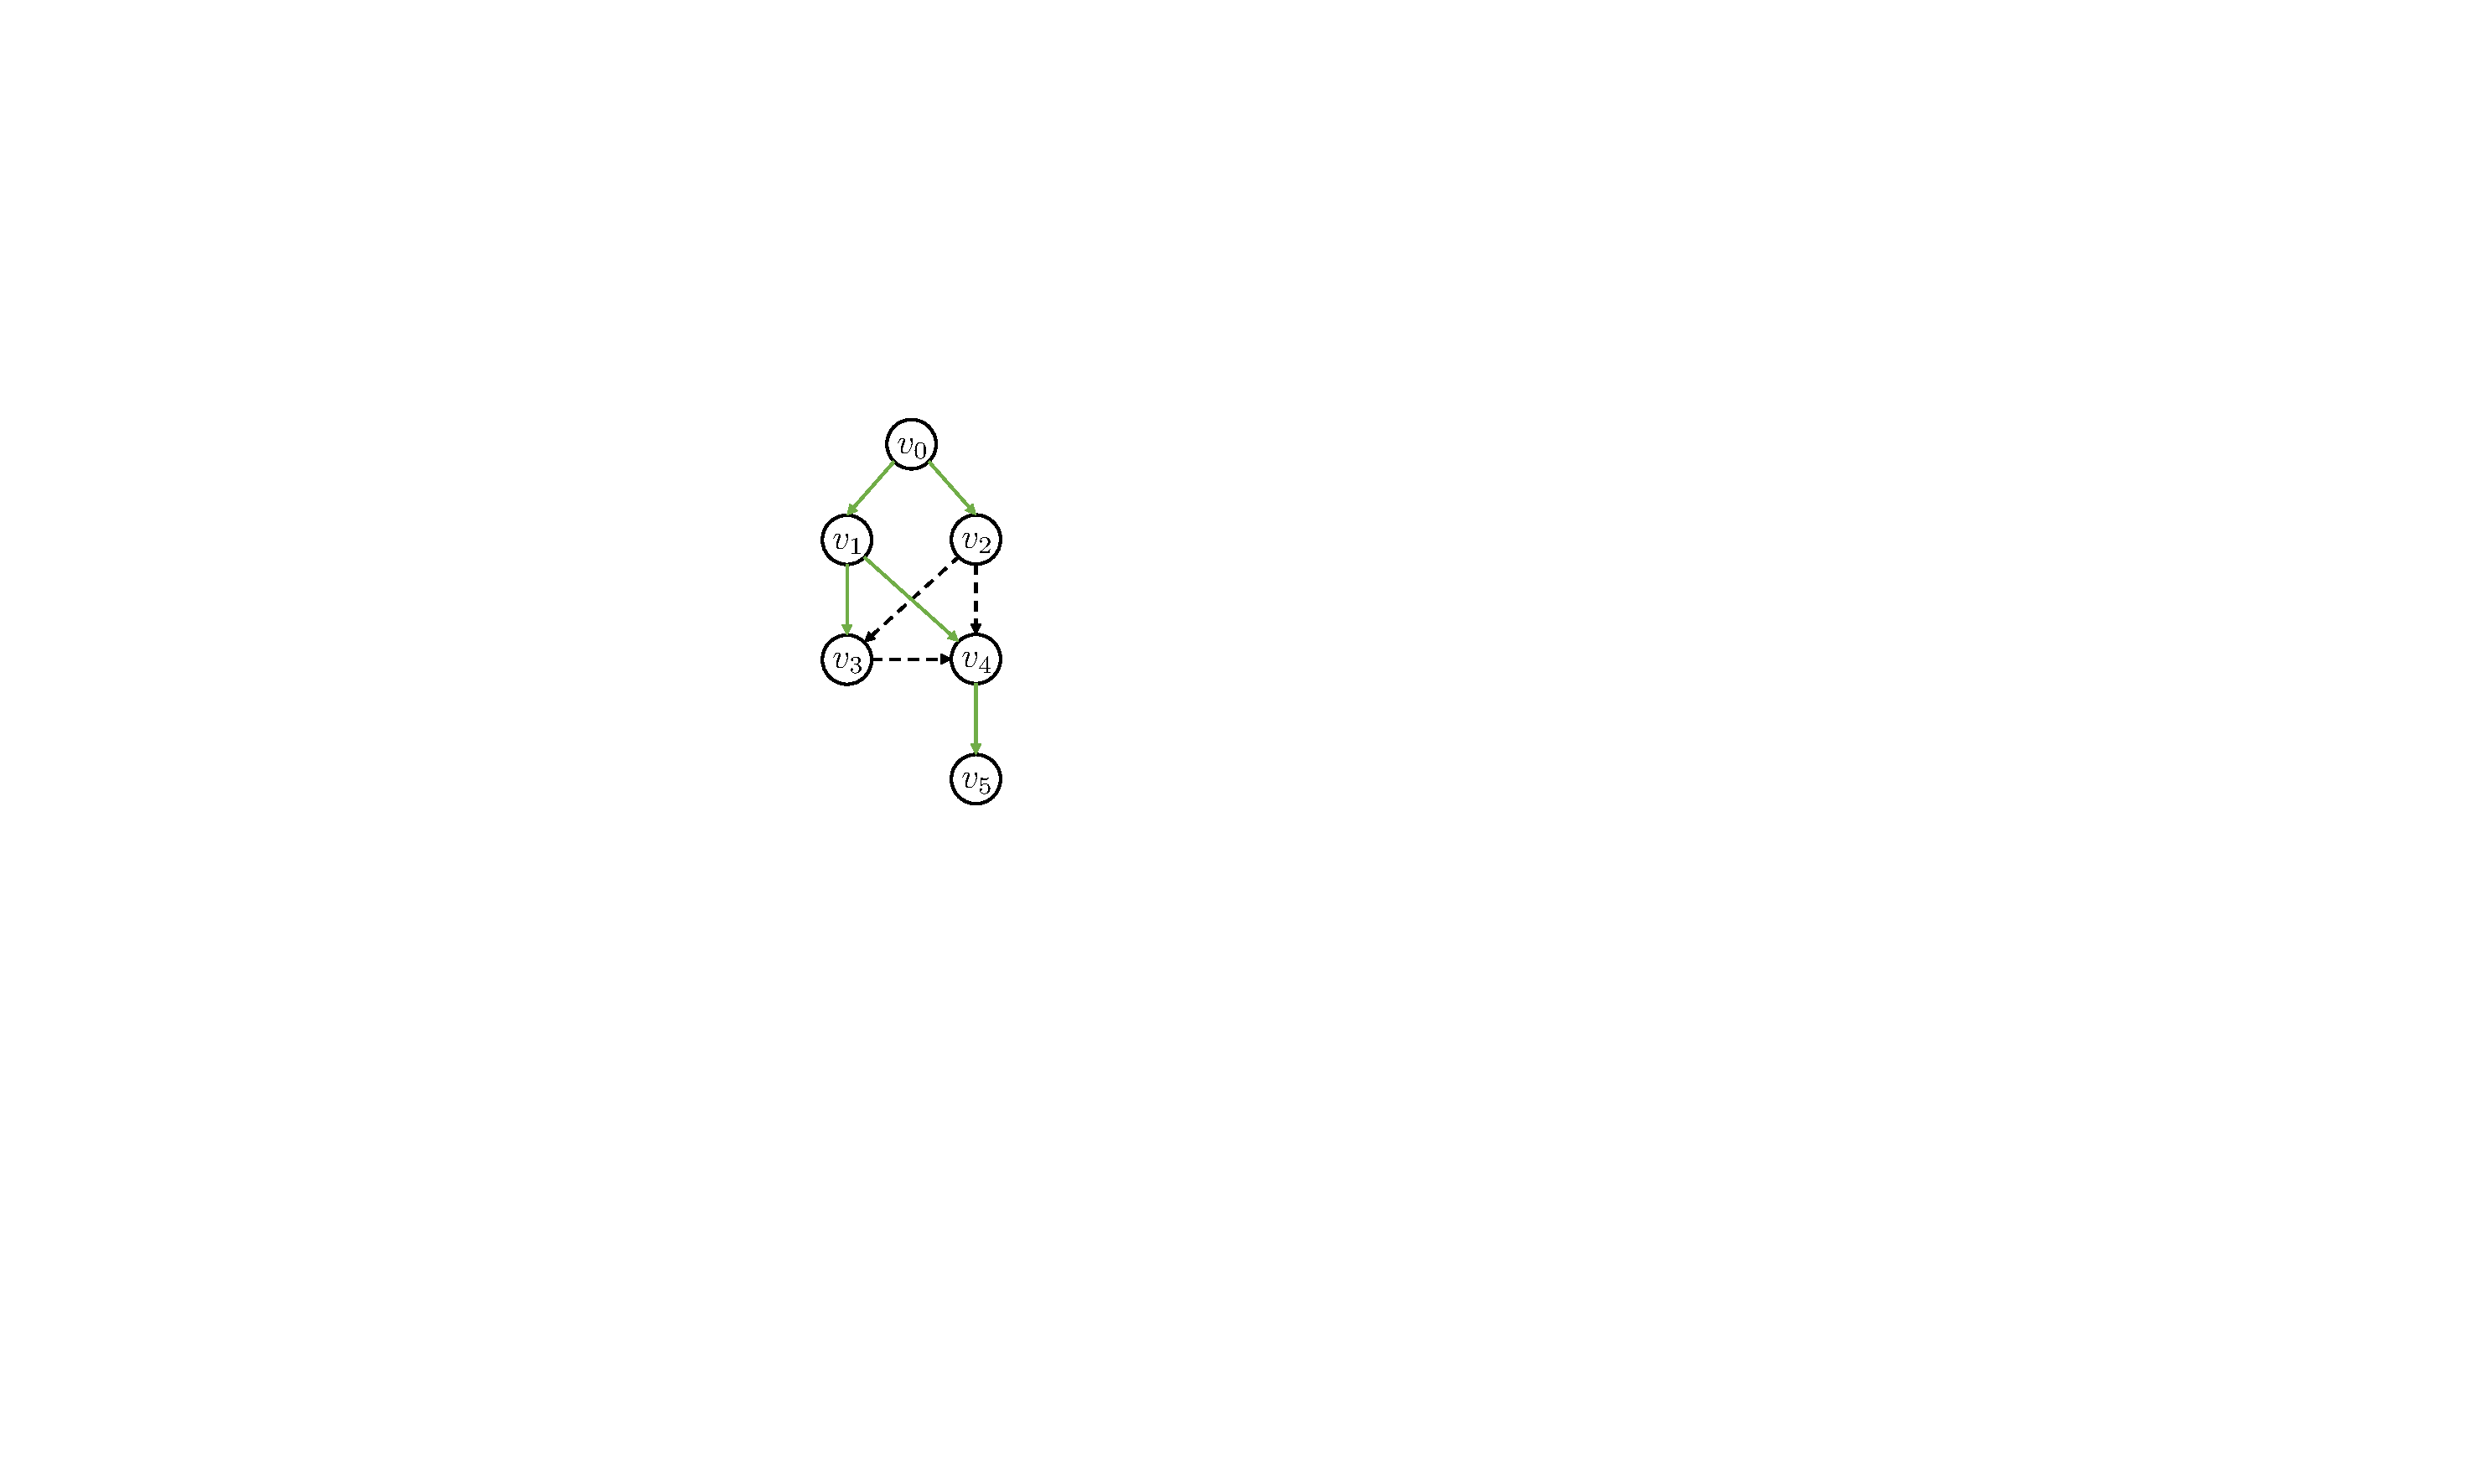
\includegraphics[clip,width=\textwidth]{figures/edge_type_b_new.pdf}
\subcaption{BFS}
\label{subfig:edge_type_b}
\end{subfigure}
\hfill
\begin{subfigure}{.3\columnwidth}
\captionsetup{width=.9\linewidth}
        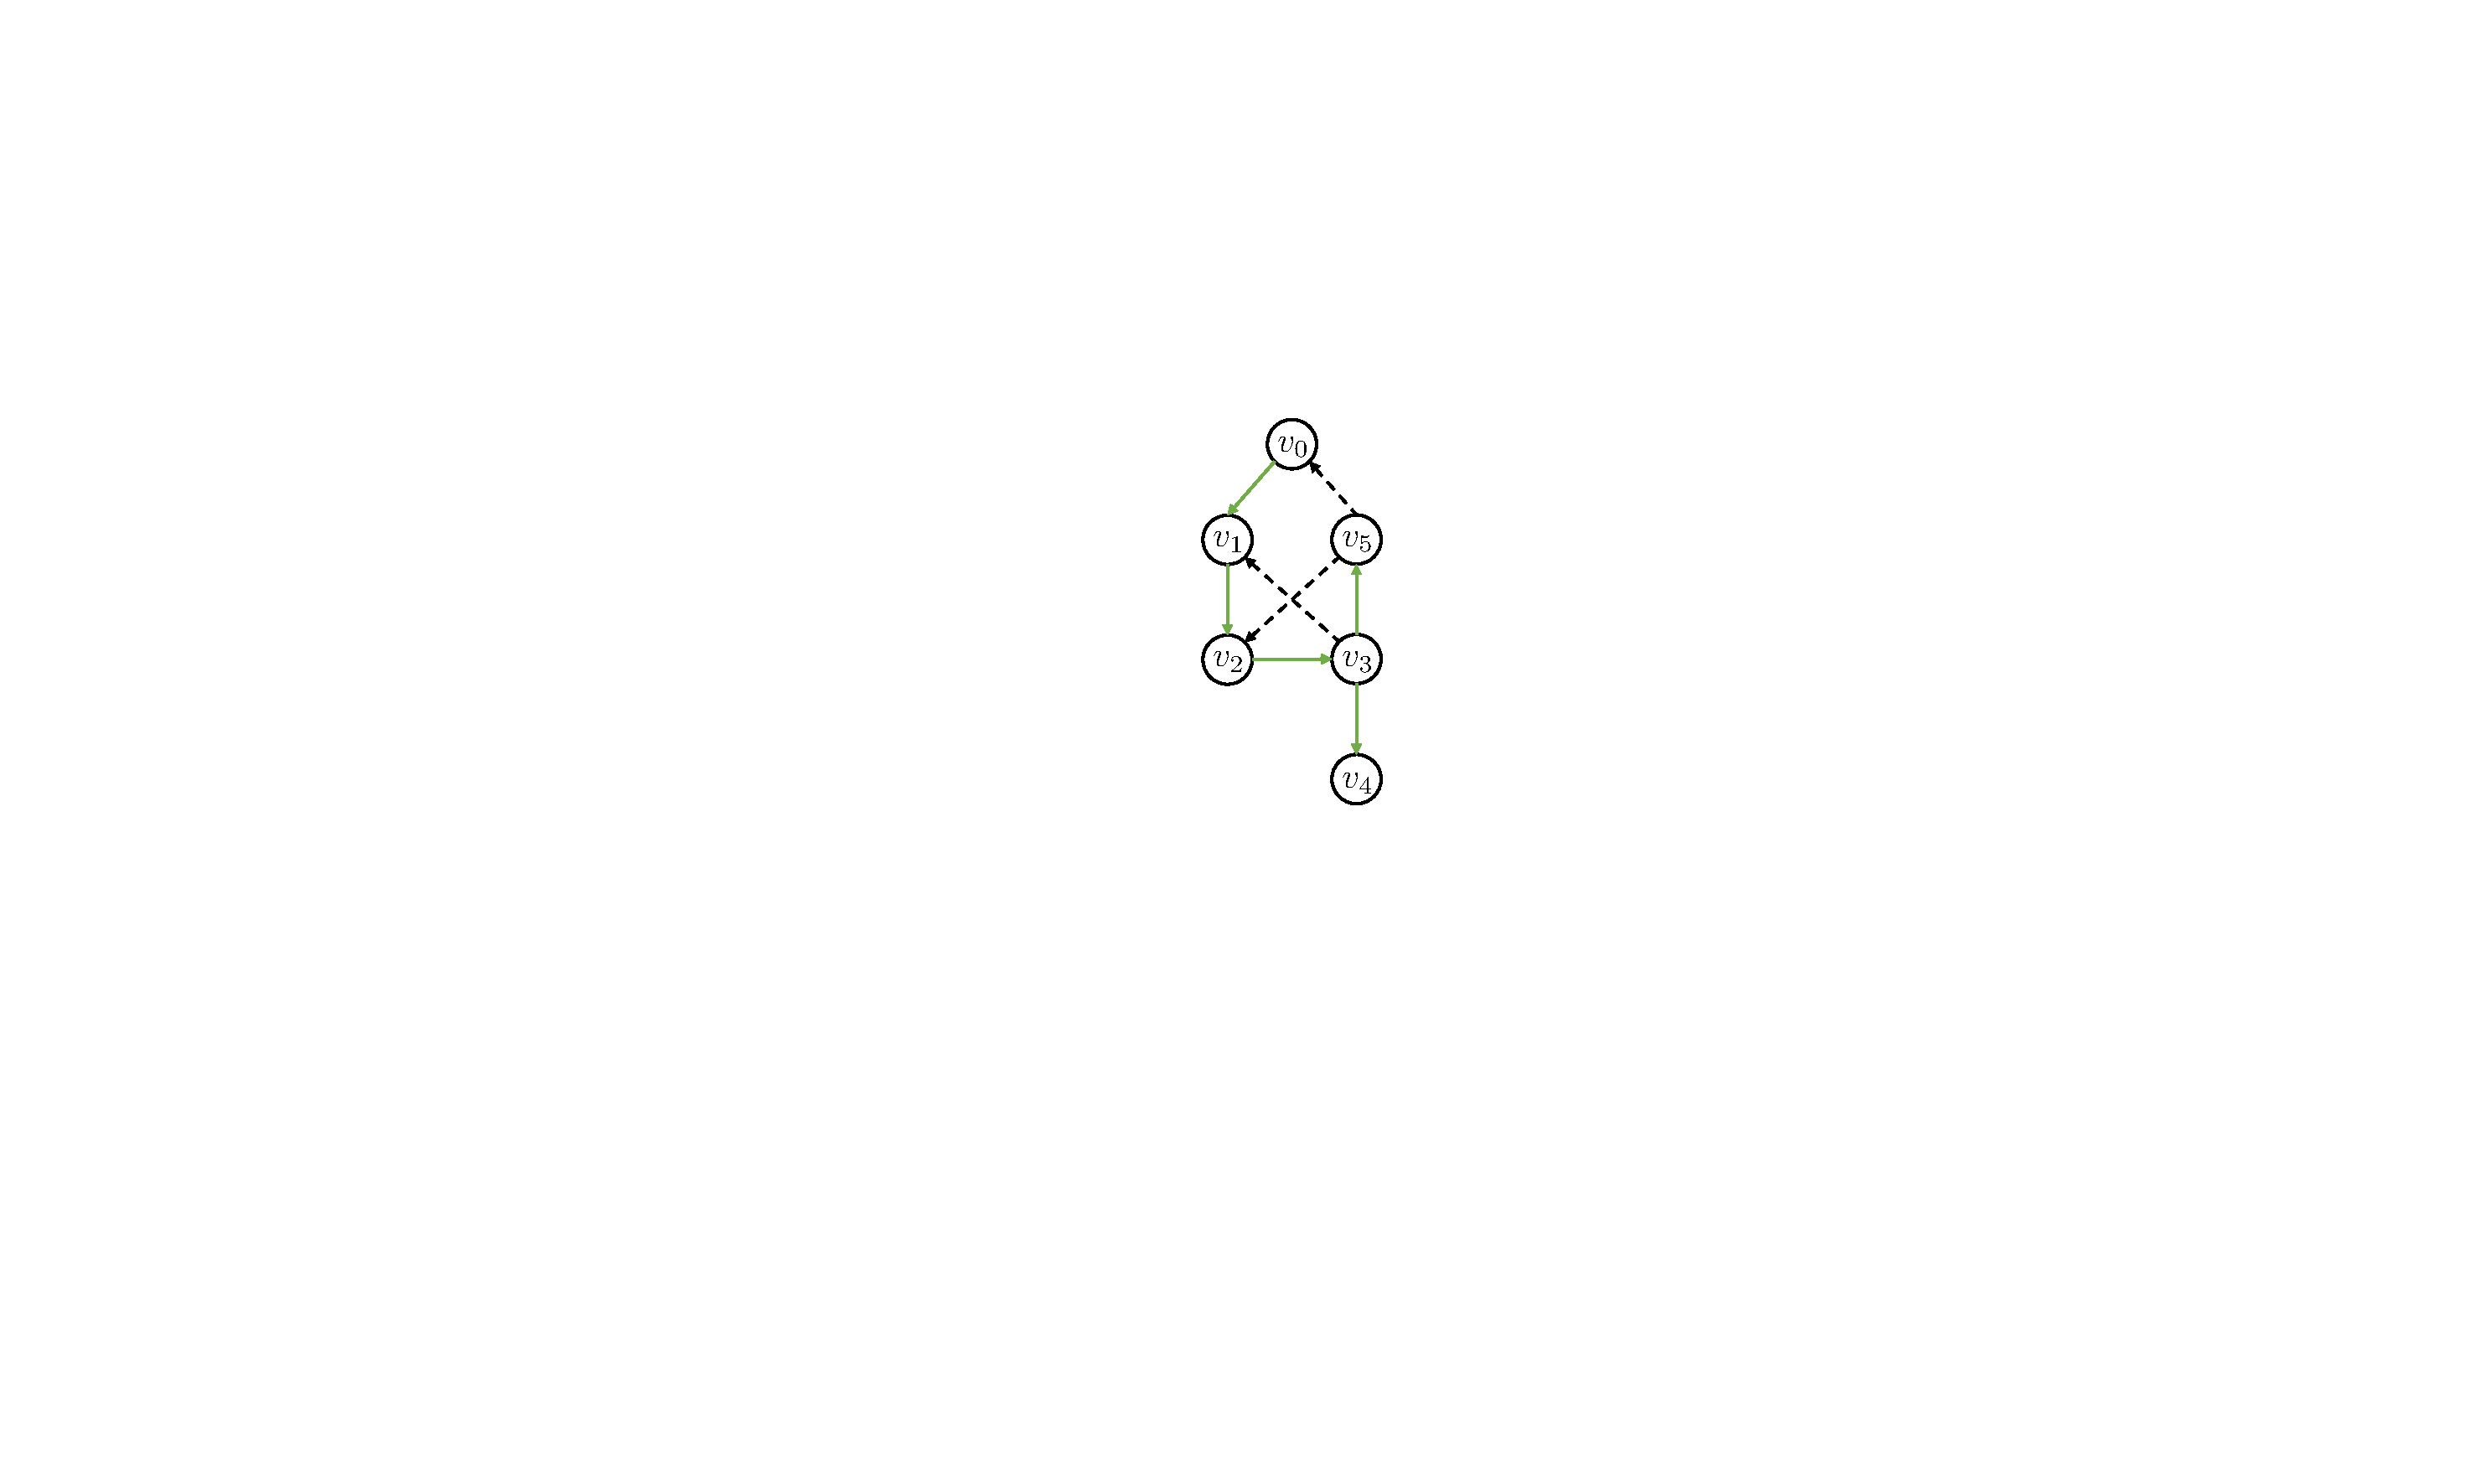
\includegraphics[clip,width=\textwidth]{figures/edge_type_c_new.pdf}
\subcaption{DFS}
\label{subfig:edge_type_c}
\end{subfigure}
\caption{Tree edges (green solid lines) and back edges (black dashed lines) classified by BFS and DFS. The subscripted labels $v_0$, \dots, $v_5$ denote the visit sequence of each vertex, e.g. $v_1$ is visited after $v_0$.}
\label{fig:edge_type}
\end{figure}